\chapter{Background}
% The background section introduces the necessary background to understand your
% work. This is not necessarily related work but technologies and dependencies
% that must be resolved to understand your design and implementation.
% This section is usually 3-5 pages.

\section{The Java Virtual Machine}
Following the "write once, run anywhere" adage, the typical way of running a Java application is with a Java Virtual Machine~(JVM).
The JVM offers an additional, target independent, layer of abstraction between implementation of 
the Java programming language~\cite{noauthor_java_nodate-2} and the operating system itself.
The JVM, is responsible for interpreting and executing Java code. It consists in four key components: 
the class loader, to load classes into memory, the runtime data area, to store program data (that is the method area, heap, and stack), the execution engine, which reads and executes bytecode instructions, and the garbage collector. The JVM Specifications~\cite{noauthor_java_nodate-1} describe in details the requirements for a JVM. 
This thesis focuses on a particular implementation, mainly Oracle's Java HotSpot~\cite{noauthor_hotspot_nodate} and its Just-In-Time~(JIT) compiler. 
HotSpot relies on tiered compilation to optimize code execution. It consists of an interpreter, and two JIT compilers: C1 and C2. 
C1 compiles bytecode with a minimal time and space overhead, applying only a limited set of optimizations, while C2 employs a more aggressive optimization strategy, requiring more resources.
The VM starts by interpreting the bytecodes to minimize startup time, and collects profiling information at the same time. Using these information, when method is deemed "hot" enough, C1 kicks in and starts compiling it. Once a threshold has been crossed C2 
recompiles the same code into a more optimized form. If an optimization is proven wrong, the code is 
deoptimized and the compiler reverts back to interpretations.  

\section{GraalVM}
GraalVM is a runtime ecosystem developed by Oracle Labs, and consists in two main components: the Graal compiler, and Native Image.
Graal is a JIT compiler that relies on multiple Phases, optimizations algorithms, to compile code 
includes multiple optimization algorithms (called “Phases”), like aggressive inlining, polymorphic inlining
 partial-escape-analysis optimization
 leverages profile-guided optimization techniques to identify hotspots in the code
complements or replaces the existing compilers (C2 in HotSpot).
 supports polyglot compilation, allowing it to compile code written in multiple programming languages supported by GraalVM, such as JavaScript, Python, Ruby using intermediate representation (IR)

Native Image\cite{noauthor_native_nodate, noauthor_native_nodate-1, wimmer_initialize_2019} is a compilation technology that compiles Java programs ahead-of-time into native binaries. It operates under a closed-world assumption, this means that all Java classes must be known at image build time to be included in the image. 
More precisely, every reflectively-accessed element, i.e, Class, Executable, and Field must be provided as reachability metadata. 
At build time, point-to-analysis is leveraged iteratively such that only reachable code remains in the final image. Initialization code of the application can run at build time instead of at run time. This two processes
reduce the startup time and memory footprint of the image.


% # Matthieu Bovel
% GraalVM is a runtime developed by Oracle Labs made of several interconnected components. The main ones are:
% • The Graal compiler is the core of the system. It consists of 1. an intermediate representation (IR) allowing
% speculative optimizations [3], 2. many optimization passes that can be applied to it and 3. the necessary
% machinery to lower it to x86 64-bit machine code. It can either integrate with HotSpot/OpenJDK, serving
% as a top-tier just-in-time compiler (replacing C2), or with native image for ahead-of-time compilation. We
% present the Graal IR in section 2.2.

\section{Java dynamic features}
One of the cornerstone of the Java ecosystem is its dynamic features. Jar, resources, proxy can be loaded, methods can be invoked at runtime, without the compiler having seen them before. 

\subsection{Dynamic class loading}
Dynamic class loading as defined in Java requires the ability to handle a sequence of bytecodes representing a class unseen by the compiler before, at runtime allows to install software componenetsw at runtime (@see Dynamic Class Loading in the JavaTMVirtual Machine)

Class 
talk about classloaders (mention delagation model -> useful for implementation), loading, linking (verifying, preparing, and resolving) and initialisation
The defining loader of D is used to load and thereby create a class or interface denoted [JVM specs] 
There are two kinds of class loaders: the bootstrap class loader supplied by the Java Virtual Machine, and user-defined class loaders. Every user-defined class loader is an instance of a subclass of the abstract class ClassLoader. Applications employ user-defined class loaders in order to extend the manner in which the Java Virtual Machine dynamically creates classes. User-defined class loaders can be used to create classes that originate from user-defined sources. For example, a class could be downloaded across a network, generated on the fly, or extracted from an encrypted file. 
When the Java Virtual Machine asks a class loader L to locate a binary representation for a class or interface called N, L loads the class or interface C denoted by N. L may load C directly, by locating a binary representation and asking the Java Virtual Machine to derive and create C from the binary representation. Alternatively, L may load C indirectly, by delegating to another class loader which loads C directly or indirectly. 

The Java Virtual Machine uses one of three procedures to create a class or interface C denoted by the name N in the run-time constant pool of a class or interface D (D triggered the class loading):

    If N denotes either a nonarray class or an interface, and D was defined by the bootstrap class loader, then the bootstrap class loader initiates loading of C (§5.3.1).

    If N denotes either a nonarray class or an interface, and D was defined by a user-defined class loader, then that same user-defined class loader initiates loading of C (§5.3.2).

    If N denotes an array class, then the Java Virtual Machine creates an array class C denoted by N, in association with the defining loader of D (§5.3.3). 
with user defined class loader:
Otherwise, the Java Virtual Machine invokes the loadClass method of class ClassLoader on L, passing the name N of a class or interface. L must perform one of the following two operations to load and thereby create a class or interface C:

    The class loader L can load C directly. This is accomplished by obtaining an array of bytes that purports to represent C as a ClassFile structure (§4.1), and then invoking the method defineClass of class ClassLoader. Invoking defineClass causes the Java Virtual Machine to derive a class or interface C denoted by N from the array of bytes using L, and then to create C, via the algorithm of §5.3.5. L should use the result of defineClass as the result of loadClass.

    The class loader L can load C indirectly, by delegating the loading of C to some other class loader L'. This is accomplished by passing the argument N to an invocation of a method on L' (typically the loadClass method of class ClassLoader). L should use the result of that method as the result of loadClass.

If C has a direct superclass, the symbolic reference from C to its direct superclass is resolved using the algorithm of §5.4.3.1. 

Linking a class or interface involves verifying and preparing that class or interface, its direct superclass, its direct superinterfaces, and its element type (if it is an array type), if necessary. Linking also involves resolution of symbolic references in the class or interface, though not necessarily at the same time as the class or interface is verified and prepared. 

This specification allows an implementation flexibility as to when linking activities (and, because of recursion, loading) take place, provided that all of the following properties are maintained:

    A class or interface is completely loaded before it is linked.

    A class or interface is completely verified and prepared before it is initialized.

    Errors detected during linkage are thrown at a point in the program where some action is taken by the program that might, directly or indirectly, require linkage to the class or interface involved in the error.

    A symbolic reference to a dynamically-computed constant is not resolved until either (i) an ldc, ldc_w, or ldc2_w instruction that refers to it is executed, or (ii) a bootstrap method that refers to it as a static argument is invoked.

    A symbolic reference to a dynamically-computed call site is not resolved until a bootstrap method that refers to it as a static argument is invoked.


%% copied from StackOverflow!
\begin{figure}
    \centering
    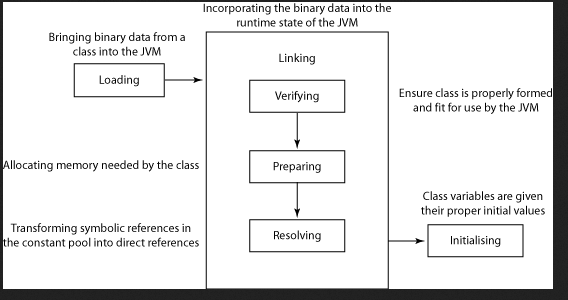
\includegraphics[width=1\linewidth]{resources/class_loading.png}
    \caption{Enter Caption}
    \label{fig:enter-label}
\end{figure}

In Java, a class is initialized when it is first used. Native Image, can initialize them at build time, as a result using the class ata runtime does not re-trigger class initialization.

\subsubsection{Java implementation}
In Java, a class is initialized when it is first used.
\subsubsection{Native Image implementation}
Every Java class used at build time is said to be build-time initialized. Note that merely loading a class does not necessarily initialize it. The static class initializer of build-time initialized classes executes on the JVM running the image build. If a class is initialized at build time, its static fields are saved in the produced binary. At run time, using such a class for the first time does not trigger class initialization.

Static analysis is a process that determines which program elements (classes, methods and fields) are used by an application. These elements are also referred to as reachable code. The analysis itself has two parts:

Scanning the bytecodes of a method to determine what other elements are reachable from it.
Scanning the root objects in the native image heap (i.e., static fields) to determine which classes are reachable from them. It starts from the entry points of the application (i.e., the main method). The newly discovered elements are iteratively scanned until further scanning yields no additional changes in element’s reachability.
Only reachable elements are included in the final image. Once a native image is built, no new elements can be added at run time, for example, through class loading. We refer to this constraint as the closed-world assumption.

\subsection{The invokedynamic instruction}
~\cite{rose_bytecodes_2009}
Talk about the usage, Method Handles, CallSites and BootStrap methods and how it required dynamic class loading
The JVM invokedynamic instruction was introduced in Java 7. It makes it possible to resolve method calls dynamically at runtime. method dispatch process by using a user-defined bootstrap method that computes the call target.
The above example uses a LambdaMetafactory to create a CallSite that is used to invoke the target method. It uses a MethodHandles.Lookup to find the target method.
The runtime approach is usually reflection-based and, consequently, inefficient. On the other hand, the compile-time solution is generally relying on code generation at compile-time. 
-> what are the case where it should throw bevaue it interprets user code?

https://docs.oracle.com/javase/specs/jvms/se21/html/jvms-5.html#jvms-5.4.3.6
To resolve an unresolved symbolic reference R to a dynamically-computed constant or call site, there are three tasks. First, R is examined to determine which code will serve as its bootstrap method, and which arguments will be passed to that code. Second, the arguments are packaged into an array and the bootstrap method is invoked. Third, the result of the bootstrap method is validated, and used as the result of resolution.

The first task involves the following steps:

    R gives a symbolic reference to a bootstrap method handle. The bootstrap method handle is resolved (§5.4.3.5) to obtain a reference to an instance of java.lang.invoke.MethodHandle.

    Any exception that can be thrown as a result of failure of resolution of a symbolic reference to a method handle can be thrown in this step.

    If R is a symbolic reference to a dynamically-computed constant, then let D be the type descriptor of the bootstrap method handle. (That is, D is a reference to an instance of java.lang.invoke.MethodType.) The first parameter type indicated by D must be java.lang.invoke.MethodHandles.Lookup, or else resolution fails with a BootstrapMethodError. For historical reasons, the bootstrap method handle for a dynamically-computed call site is not similarly constrained.

    If R is a symbolic reference to a dynamically-computed constant, then it gives a field descriptor.

    If the field descriptor indicates a primitive type, then a reference to the pre-defined Class object representing that type is obtained (see the method isPrimitive in class Class).

    Otherwise, the field descriptor indicates a class or interface type, or an array type. A reference to the Class object representing the type indicated by the field descriptor is obtained, as if by resolution of an unresolved symbolic reference to a class or interface (§5.4.3.1) whose name corresponds to the type indicated by the field descriptor.

    Any exception that can be thrown as a result of failure of resolution of a symbolic reference to a class or interface can be thrown in this step.

    If R is a symbolic reference to a dynamically-computed call site, then it gives a method descriptor.

    A reference to an instance of java.lang.invoke.MethodType is obtained, as if by resolution of an unresolved symbolic reference to a method type (§5.4.3.5) with the same parameter and return types as the method descriptor.

    Any exception that can be thrown as a result of failure of resolution of a symbolic reference to a method type can be thrown in this step.


invokedynamic is a bytecode operation used to call arbitrary method within JVM. The exact method to be called and executed is unknown at a compile-time. Instead it is computed by object implementing CallSite. Thus the dynamic in invokedynamic.

CallSite objects, as any other, have to be instantiated. Boostrap Method is a method which instantiates CallSite objects.

Each invokedynamic has a known bootstrap method given as its compile-time parameter. Whenever a invokedynamic is processed for a first time, appropriate bootstrap method is invoked. As result of boostrap method execution a CallSite object is created. This CallSite object is then cached and associated by JVM to a given invokedynamic operation. From now on, whenever particular invokedynamic call is to be executed, a cached CallSite instance is used to resolve called method.

Majority of boostrap methods are not written directly by end Java programmer. However that doesn't mean they are some rare obscure mechanism. They are created by javac compiler whenever particular java statements are used within source. String concatenation or lambda expression come to mind.

For example lambda expression could be implemented as inner classes. For matter of fact, lambdas are presented to programmers 'as shorthand' to using inner classes. However actual javac implementation, for performance reasons, avoids inner classes by generating lambda code under a static method and using invokedynamic to invoke this method.
\subsubsection{Java implementation}
Talk about the bootstrap method invokers, invokers, lanbdametafactory and altmetafactory and lambdaforms -> interpretation until the lambdaform is
considered to be hot enough to be compiled, customized, uncustomized if needed, cf tiered compilation
\subsubsection{Native Image implementaiton}
Some are compiled at image built time (indy and trusted condy BSM), the other are forced interpreted


\section{Reflection}

\subsubsection{Java implementation}

\subsubsection{Native Image implementation}
Reachability Metadata and Tracing Agent

 